%%%%%%%%%%%%%%%%%%%%%%%%%%% asme2ej.tex %%%%%%%%%%%%%%%%%%%%%%%%%%%%%%%
% Template for producing ASME-format journal articles using LaTeX    %
% Written by   Harry H. Cheng, Professor and Director                %
%              Integration Engineering Laboratory                    %
%              Department of Mechanical and Aeronautical Engineering %
%              University of California                              %
%              Davis, CA 95616                                       %
%              Tel: (530) 752-5020 (office)                          %
%                   (530) 752-1028 (lab)                             %
%              Fax: (530) 752-4158                                   %
%              Email: hhcheng@ucdavis.edu                            %
%              WWW:   http://iel.ucdavis.edu/people/cheng.html       %
%              May 7, 1994                                           %
% Modified: February 16, 2001 by Harry H. Cheng                      %
% Modified: January  01, 2003 by Geoffrey R. Shiflett                %
% Butchered: October 15, 2014 by John Karasinski                     %
% Use at your own risk, send complaints to /dev/null                 %
%%%%%%%%%%%%%%%%%%%%%%%%%%%%%%%%%%%%%%%%%%%%%%%%%%%%%%%%%%%%%%%%%%%%%%

%%% use twocolumn and 10pt options with the asme2ej format
\documentclass[twocolumn,10pt]{asme2ej}

\usepackage{epsfig} %% for loading postscript figures
\usepackage{amsmath}
\usepackage{graphicx}
\usepackage{grffile}
\usepackage{pdfpages}
\usepackage{algpseudocode}

% Default fixed font does not support bold face
\DeclareFixedFont{\ttb}{T1}{txtt}{bx}{n}{12} % for bold
\DeclareFixedFont{\ttm}{T1}{txtt}{m}{n}{12}  % for normal

% Custom colors
\usepackage{color}
\usepackage{listings}
\usepackage{framed}
\usepackage{caption}
\captionsetup[lstlisting]{font={small,tt}}

\definecolor{mygreen}{rgb}{0,0.6,0}
\definecolor{mygray}{rgb}{0.5,0.5,0.5}
\definecolor{mymauve}{rgb}{0.58,0,0.82}

\lstset{ %
  backgroundcolor=\color{white},   % choose the background color; you must add \usepackage{color} or \usepackage{xcolor}
  basicstyle=\ttfamily\footnotesize, % the size of the fonts that are used for the code
  breakatwhitespace=false,         % sets if automatic breaks should only happen at whitespace
  % breaklines=true,                 % sets automatic line breaking
  captionpos=b,                    % sets the caption-position to bottom
  commentstyle=\color{mygreen},    % comment style
  deletekeywords={...},            % if you want to delete keywords from the given language
  escapeinside={\%*}{*)},          % if you want to add LaTeX within your code
  extendedchars=true,              % lets you use non-ASCII characters; for 8-bits encodings only, does not work with UTF-8
  frame=single,                    % adds a frame around the code
  keepspaces=true,                 % keeps spaces in text, useful for keeping indentation of code (possibly needs columns=flexible)
  columns=flexible,
  keywordstyle=\color{blue},       % keyword style
  language=Python,                 % the language of the code
  morekeywords={*,...},            % if you want to add more keywords to the set
  numbers=left,                    % where to put the line-numbers; possible values are (none, left, right)
  numbersep=5pt,                   % how far the line-numbers are from the code
  numberstyle=\tiny\color{mygray}, % the style that is used for the line-numbers
  rulecolor=\color{black},         % if not set, the frame-color may be changed on line-breaks within not-black text (e.g. comments (green here))
  showspaces=false,                % show spaces everywhere adding particular underscores; it overrides 'showstringspaces'
  showstringspaces=false,          % underline spaces within strings only
  showtabs=false,                  % show tabs within strings adding particular underscores
  stepnumber=1,                    % the step between two line-numbers. If it's 1, each line will be numbered
  stringstyle=\color{mymauve},     % string literal style
  tabsize=4,                       % sets default tabsize to 2 spaces
}

\title{Final: Incompressible, Laminar Flow over a Rectangular Cavity}

\author{John Karasinski
    \affiliation{
  Graduate Student Researcher\\
  Center for Human/Robotics/Vehicle Integration and Performance\\
  Department of Mechanical and Aerospace Engineering\\
  University of California\\
  Davis, California 95616\\
    Email: karasinski@ucdavis.edu
    }
}

\begin{document}
\maketitle

%%%%%%%%%%%%%%%%%%%%%%%%%%%%%%%%%%%%%%%%%%%%%%%%%%%%%%%%%%%%%%%%%%%%%%
\section{Problem Description}

Forty five years ago, Mehta and Lavan published a paper on the numerical investigation of flow over a rectangular cavity at low Reynolds numbers~\cite{mehta1969flow}. This relatively simple geometry provides tremendous insight into the physics of flow separation, an important flow feature in many applications. A numerical 2D planar model of these incompressible, laminar flows is developed here. In particular, the predicted flow structure (streamline pattern, eddies) and velocity profiles are investigated for a variety of aspect ratios (AR) and Reynolds numbers (Re).

%%%%%%%%%%%%%%%%%%%%%%%%%%%%%%%%%%%%%%%%%%%%%%%%%%%%%%%%%%%%%%%%%%%%%%
\section{Numerical Solution Approach}

The icoFoam solver from OpenFOAM 2.3.0 was used to model the solution of this problem. icoFoam is a transient solver for incompressible, laminar flow of Newtonian fluid. Five cases were investigated: a base case with AR=0.5 and Reynolds number (Re) of 100, and additional cases of AR=0.5 with Re=1 and 2000 for AR=0.5, and AR=2.0 and 5.0 for Re=100. A Python script was created to generate the initial conditions and geometry for each case.

The solver is initialized with the initial conditions described in Table~\ref{initial_conditions}. Additionally, the boundary field for the inlet and outlet boundaries are set to ``zeroGradient'' for all of the initial fields and, the boundary field for frontAndBack is set to ``empty'' for all initial fields, turning this into a 2D problem. The geometry for this problem consists of a channel of width 10 m and height 1 m. A cavity is placed just below the channel and has a width of 1 m and a depth of AR (see Figure~\ref{geometry_figure}).

The script also generated the nonuniform mesh for this geometry using the blockMesh tool. This mesh was divided into four regions: the left half of the channel, the right half of the channel, the center of the channel, and the cavity. For the base case, both the left and right halves of the channel were split into grids of 50x50 in the x, y direction, and also used ``simpleGrading'' to grade the meshes to make them denser near the center of the domain. The center of the channel was also split into grids of 50x50 in the x, y direction. The cavity for the base case was split into grids of 50x25 in the x, y direction and created a uniform mesh. A generalized version of this mesh is available in Table~\ref{mesh_generation}.

The resultant mesh for the base case can be see in Figure~\ref{grid_figure}. The domain of the problem was then split on to four CPUs using the decomposePar tool, and the icoFoam solver was called with the MPI option. The solver than solved the system to convergence and reconstructed the domain using the reconstructPar tool. The system was considered converged when the flow before and after the cavity both approximated a linear function (see Figure~\ref{velocity_profile}). This accomplished by creating by sampling the flow rate at $x=$1 and $x=$-1 and plotting against y. the ``sample'' function.

\begin{table}[bt]
\begin{center}
\begin{tabular}{| l | l | l | l | }
\hline
                & internal    & lid          & fixedWalls   \\
\hline
U~[m/s]         & (0 0 0)$^*$ & (1 0 0)$^*$  & (0 0 0)$^*$  \\
p~[m$^2$/s$^2$] & 0$^*$       & zeroGradient & zeroGradient \\
\hline
\end{tabular}
\caption{Initial conditions for simulation ($^*$: uniform field)}
\label{initial_conditions}
\end{center}
\end{table}

\begin{table}[bt]
\begin{center}
\begin{tabular}{| l | r r r | }
\hline
Name            & x &  y    & simpleGrading \\
\hline
Left channel    & M &  M    & (5/M 1 1) \\
Right channel   & M &  M    & (M/5 1 1) \\
Central channel & M &  M    & (1   1 1) \\
Cavity          & M &  M*AR & (1   1 1) \\
\hline
\end{tabular}
\caption{Mesh configuration algorithm (M=50, AR=0.5 for base case)}
\label{mesh_generation}
\end{center}
\end{table}

\begin{figure}[tb]
\begin{center}
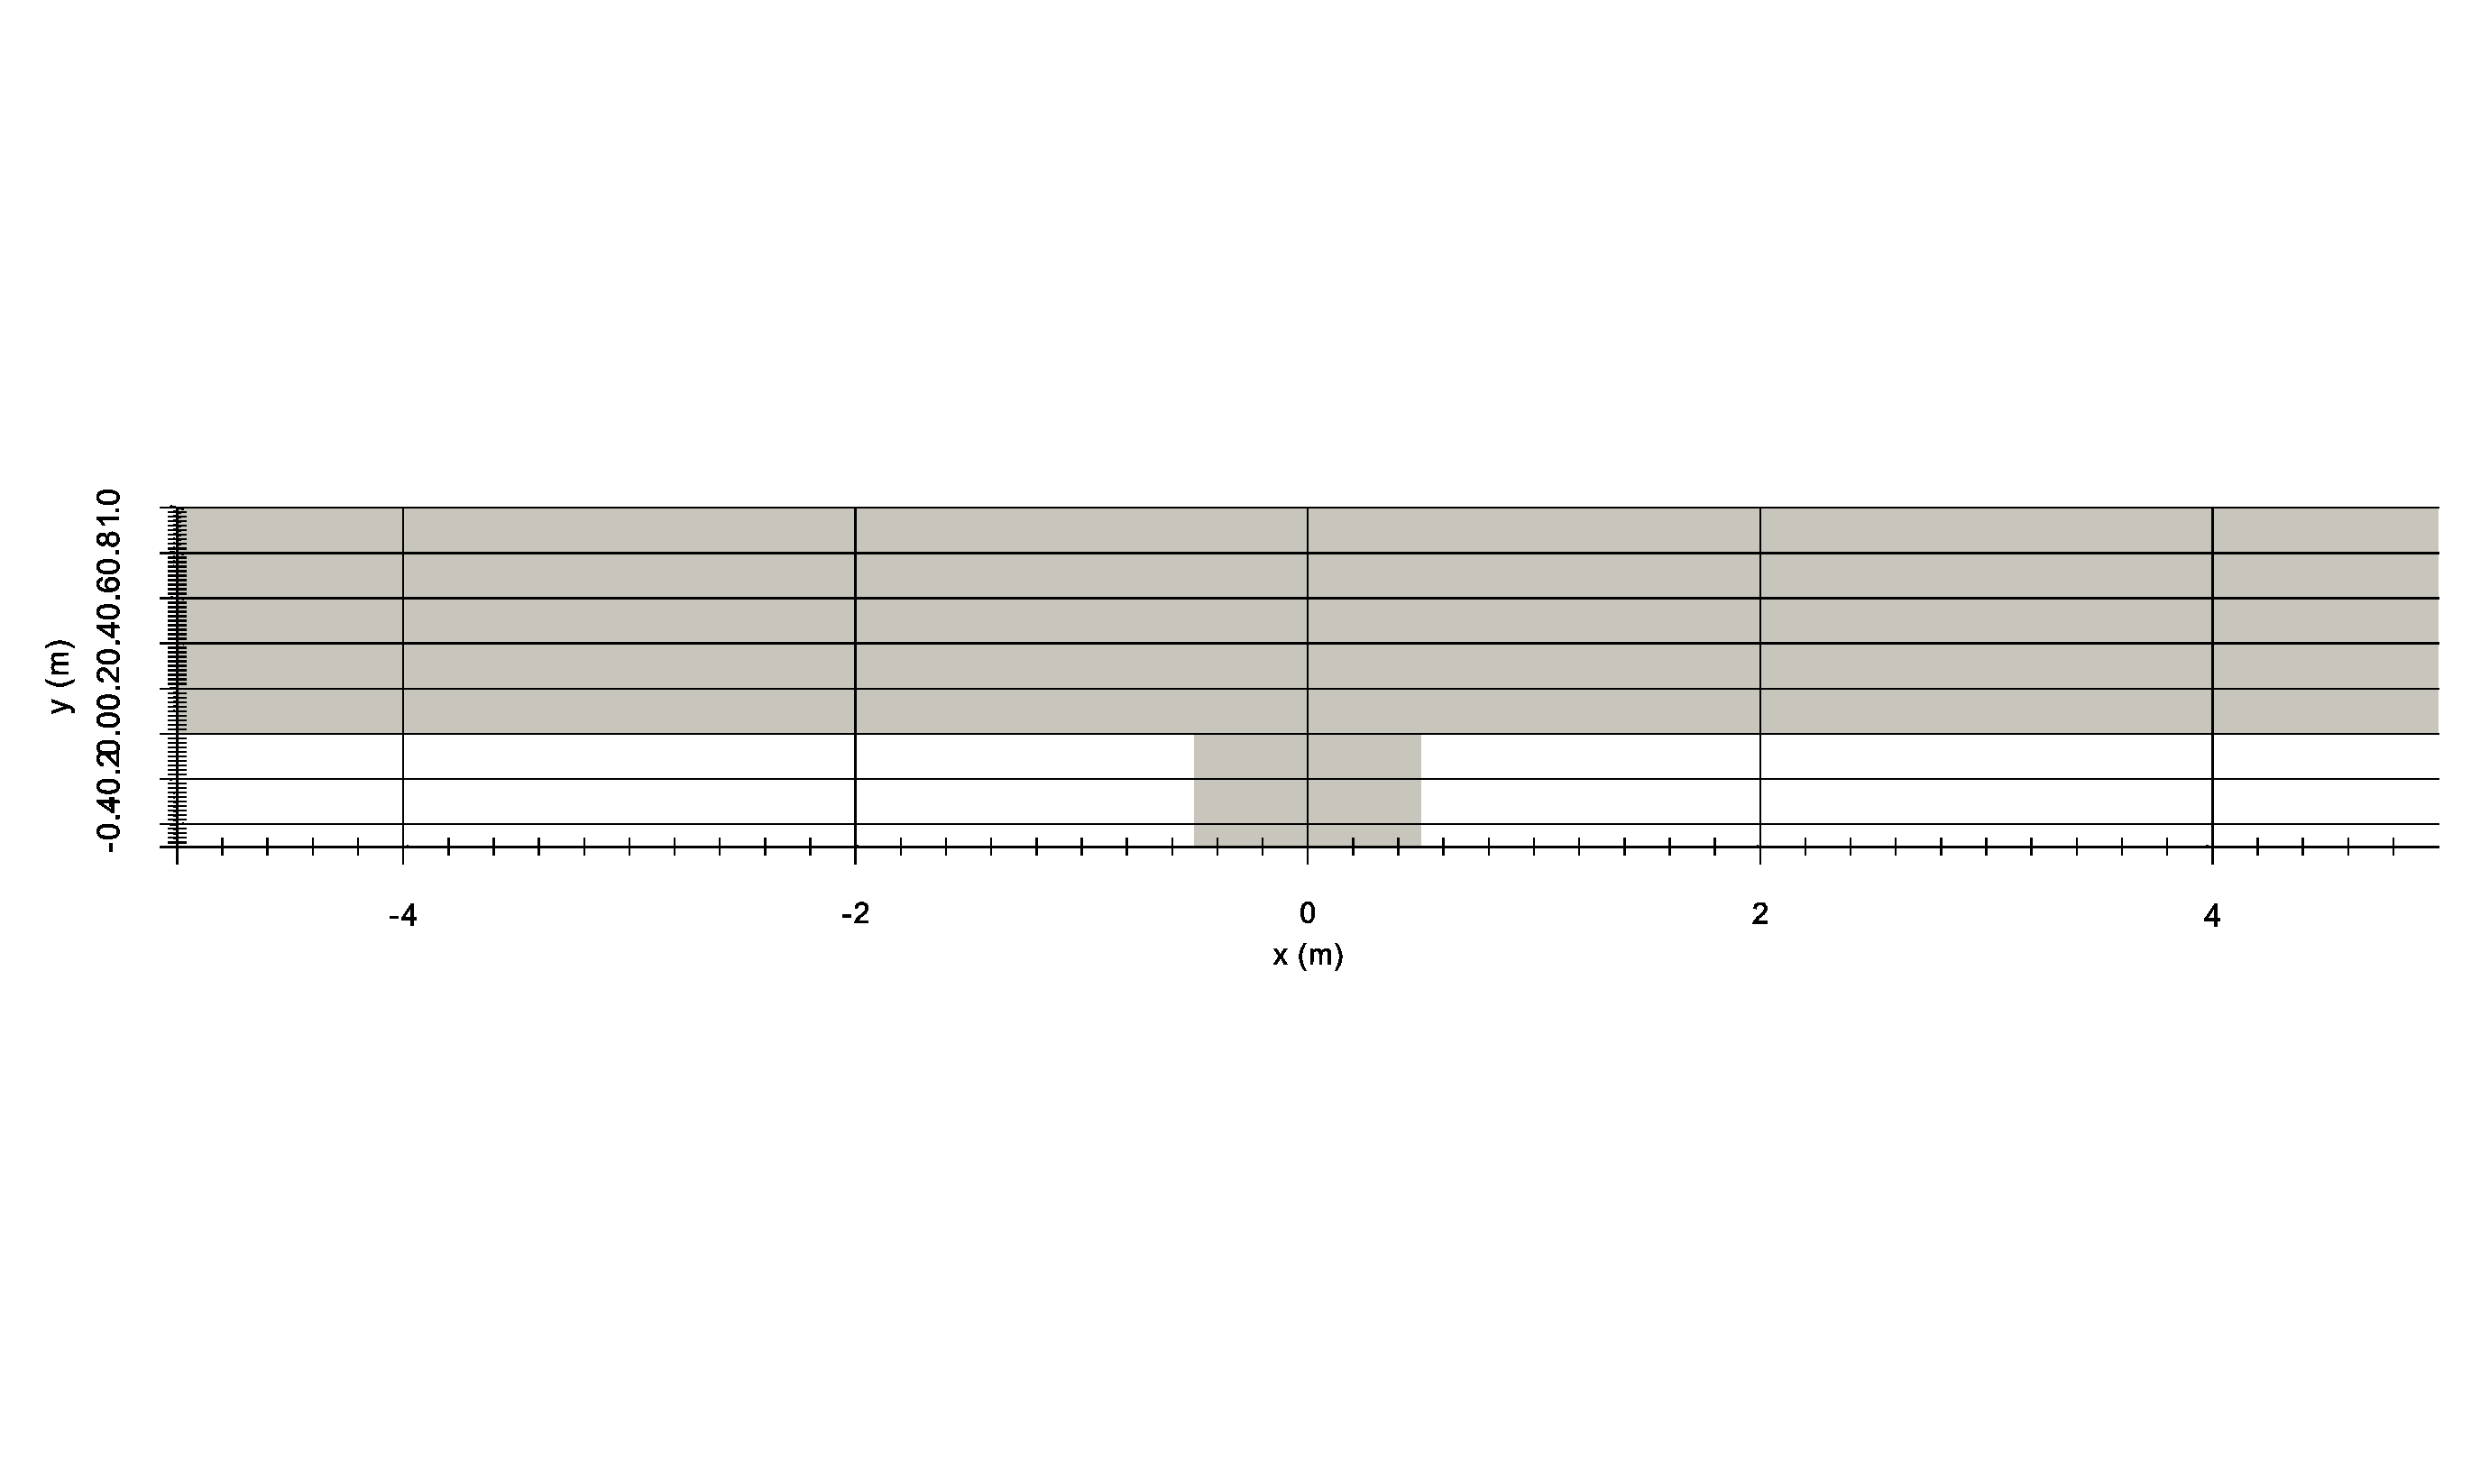
\includegraphics[width=0.5\textwidth]{figure/geometry.pdf}
\caption{Geometry for the AR=0.5 cases}
\label{geometry_figure}
\end{center}
\end{figure}

\begin{figure}[tb]
\begin{center}
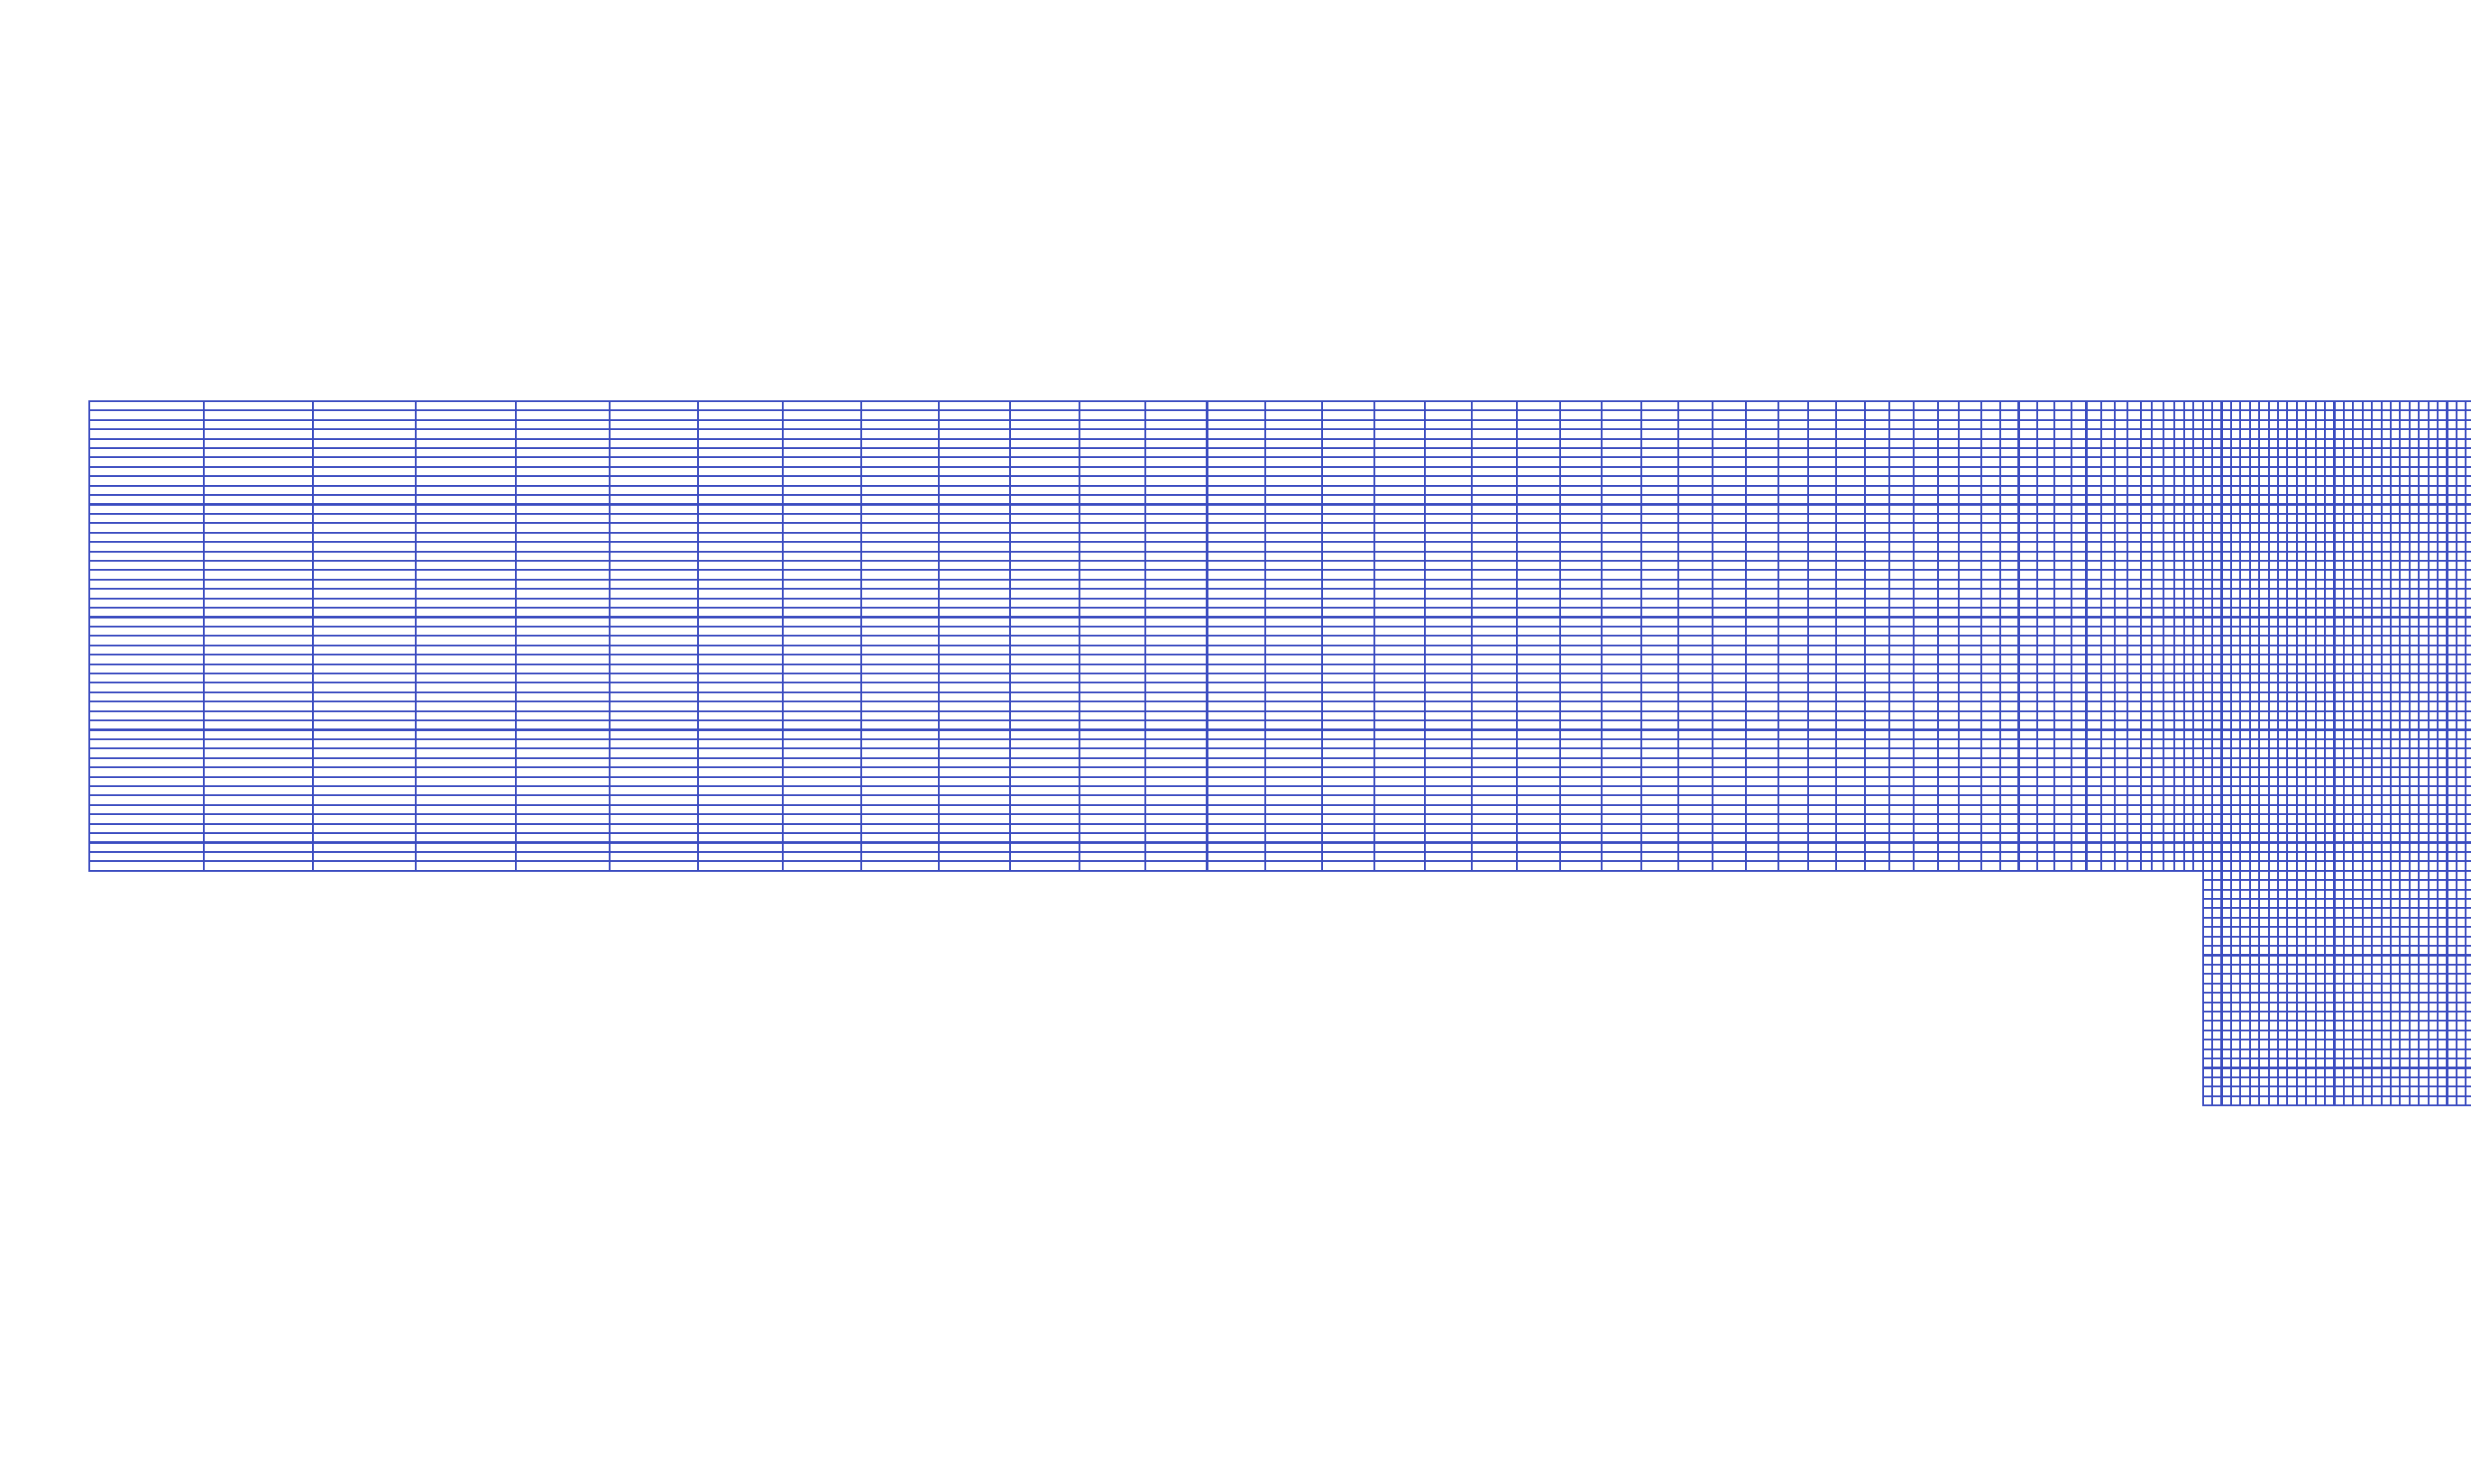
\includegraphics[width=0.5\textwidth]{figure/half_grid.pdf}
\caption{Closeup on the left half of the mesh generated for the AR=0.5 cases, showing the gradient towards the center}
\label{grid_figure}
\end{center}
\end{figure}

\begin{figure}[tb]
\begin{center}
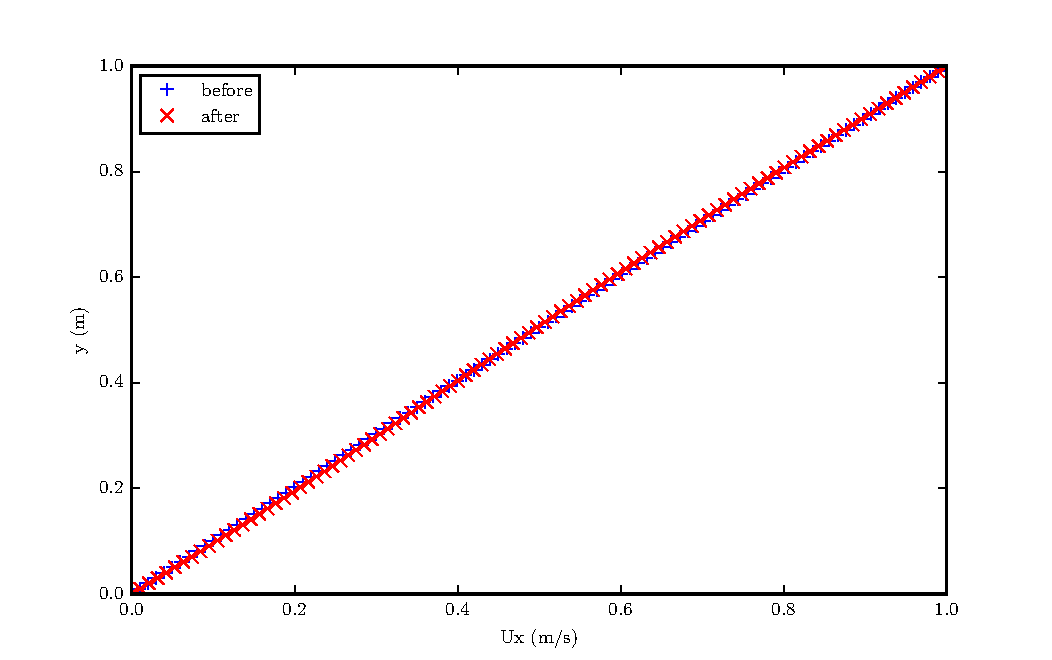
\includegraphics[width=0.5\textwidth]{figure/Ar0.5-Re100 Ux before and after.pdf}
\caption{Velocity profile of Ux before ($x = 1 $m) and after ($x = -1 $m) cavity, for base case}
\label{velocity_profile}
\end{center}
\end{figure}

\begin{figure}[tb]
\begin{center}
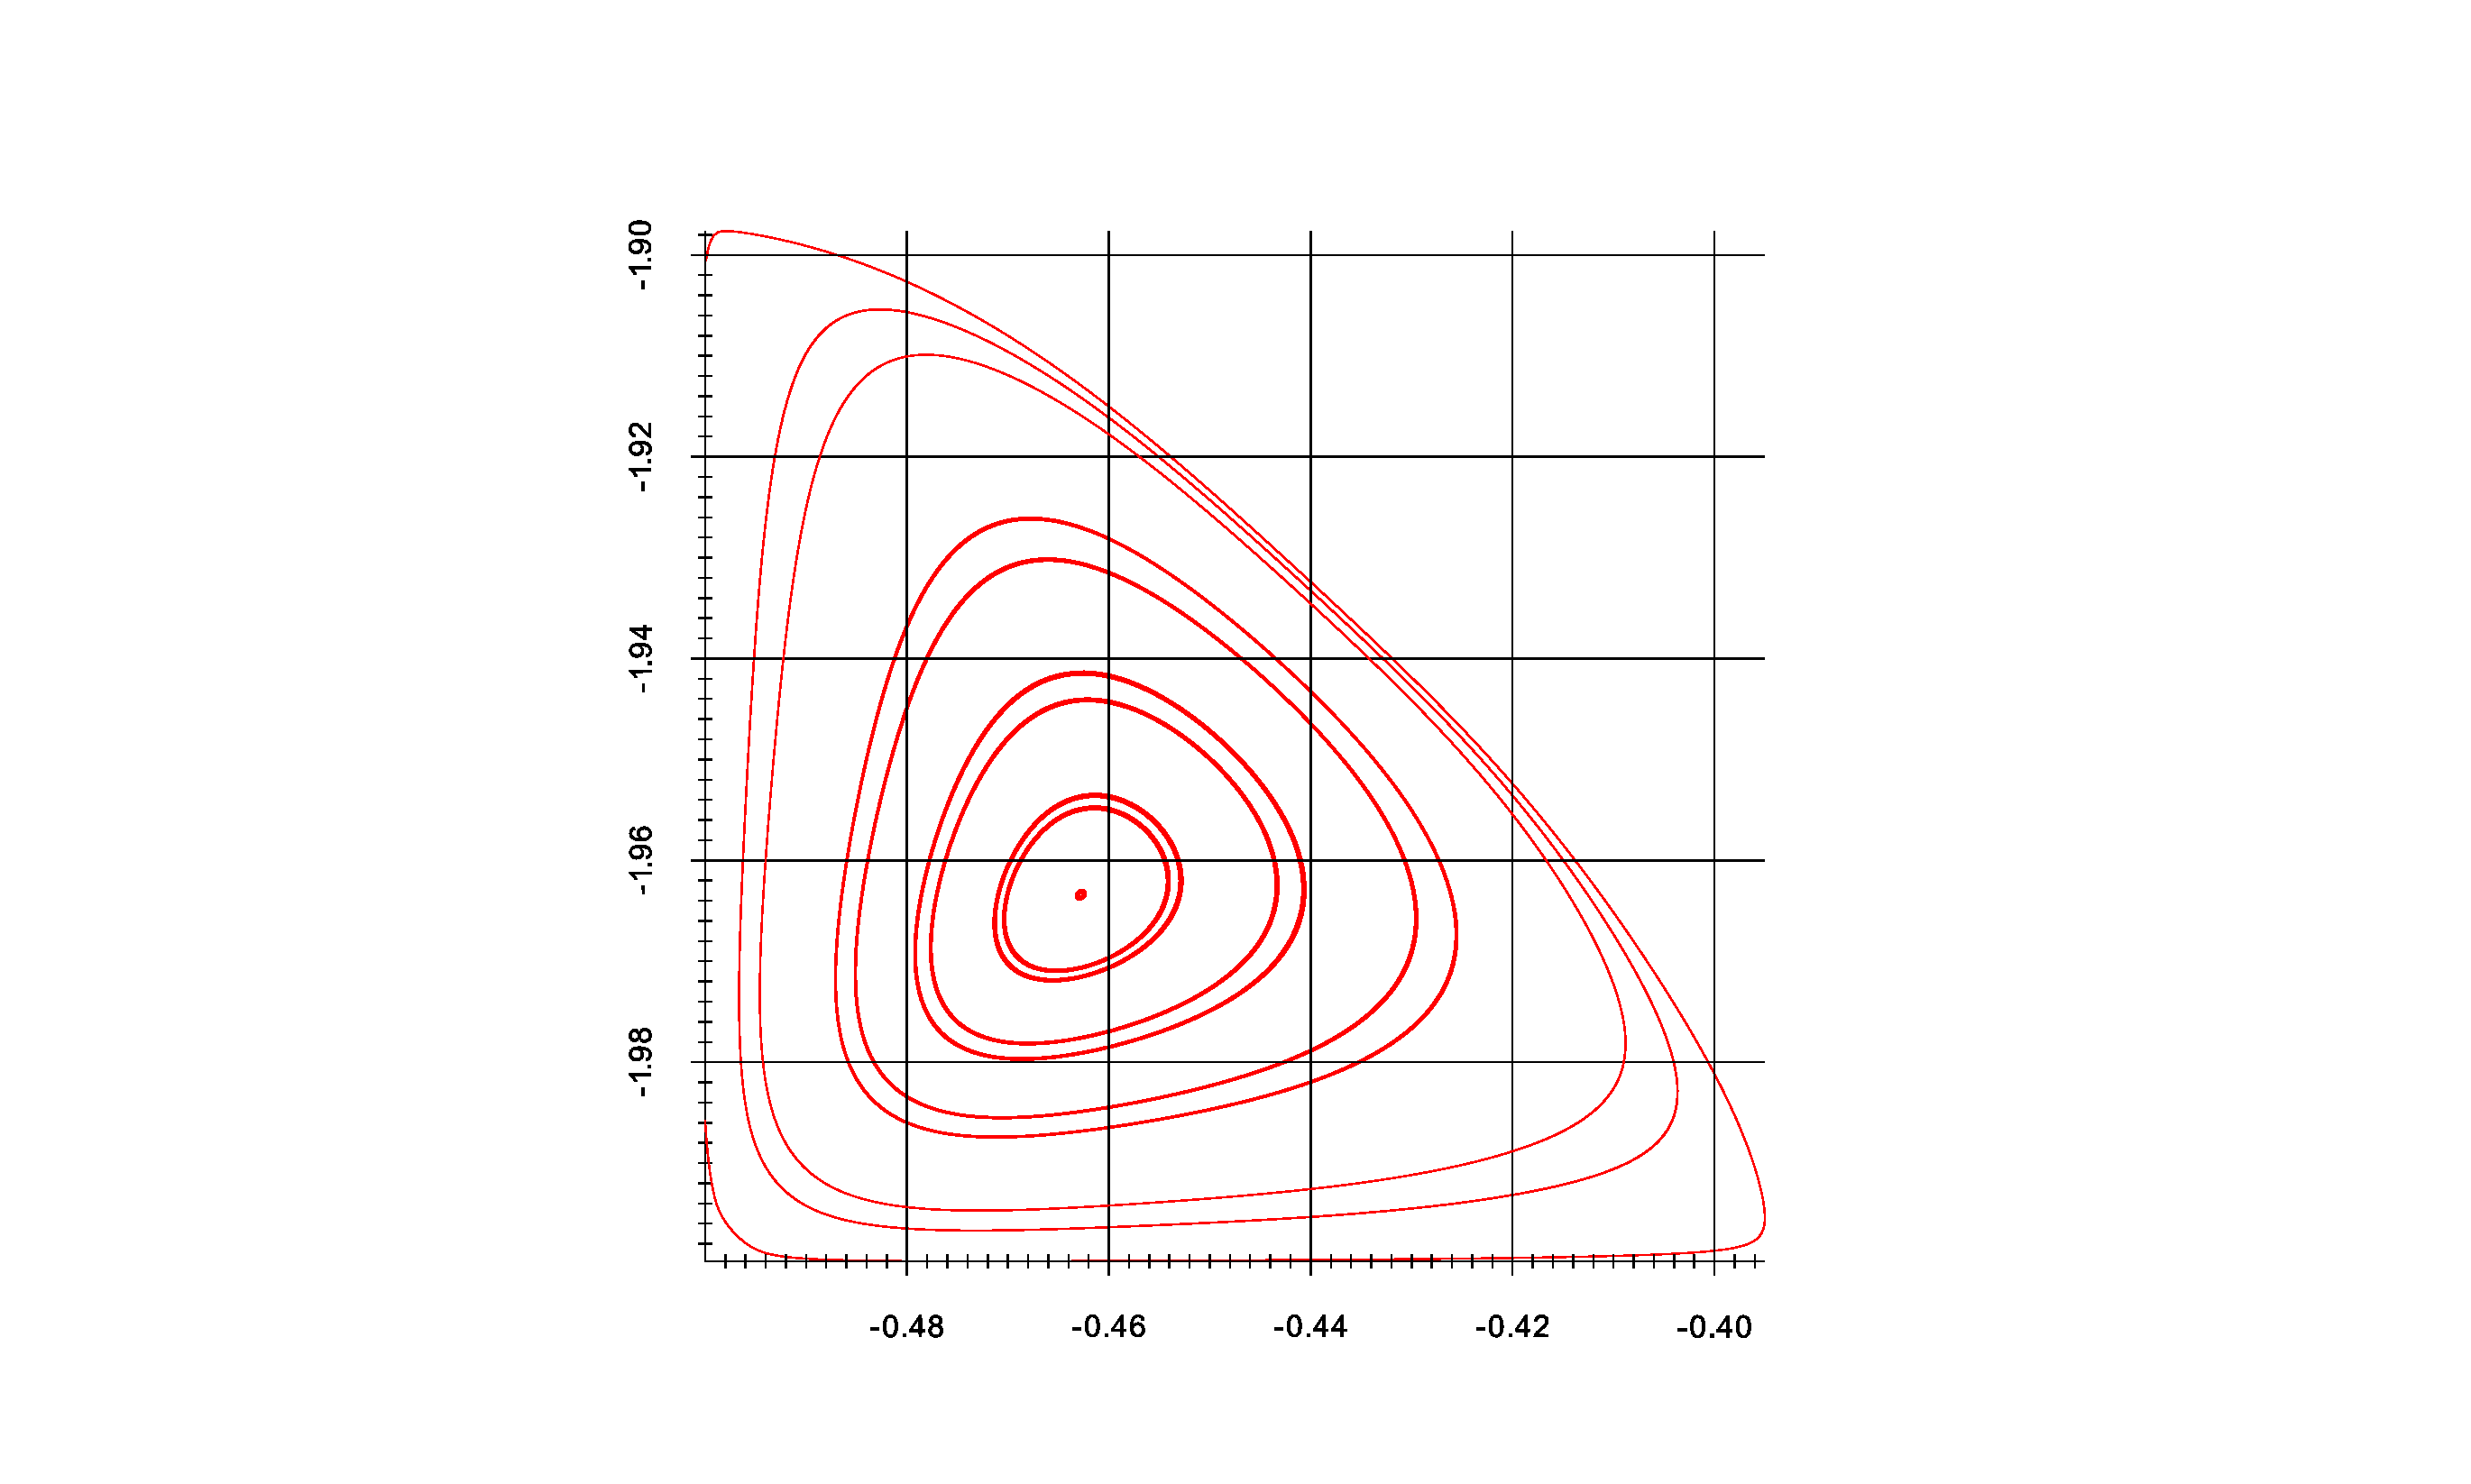
\includegraphics[width=0.5\textwidth]{figure/LeftCornerLarge.pdf}
\caption{Upstream corner eddy}
\label{velocity_profile}
\end{center}
\end{figure}

\begin{figure}[tb]
\begin{center}
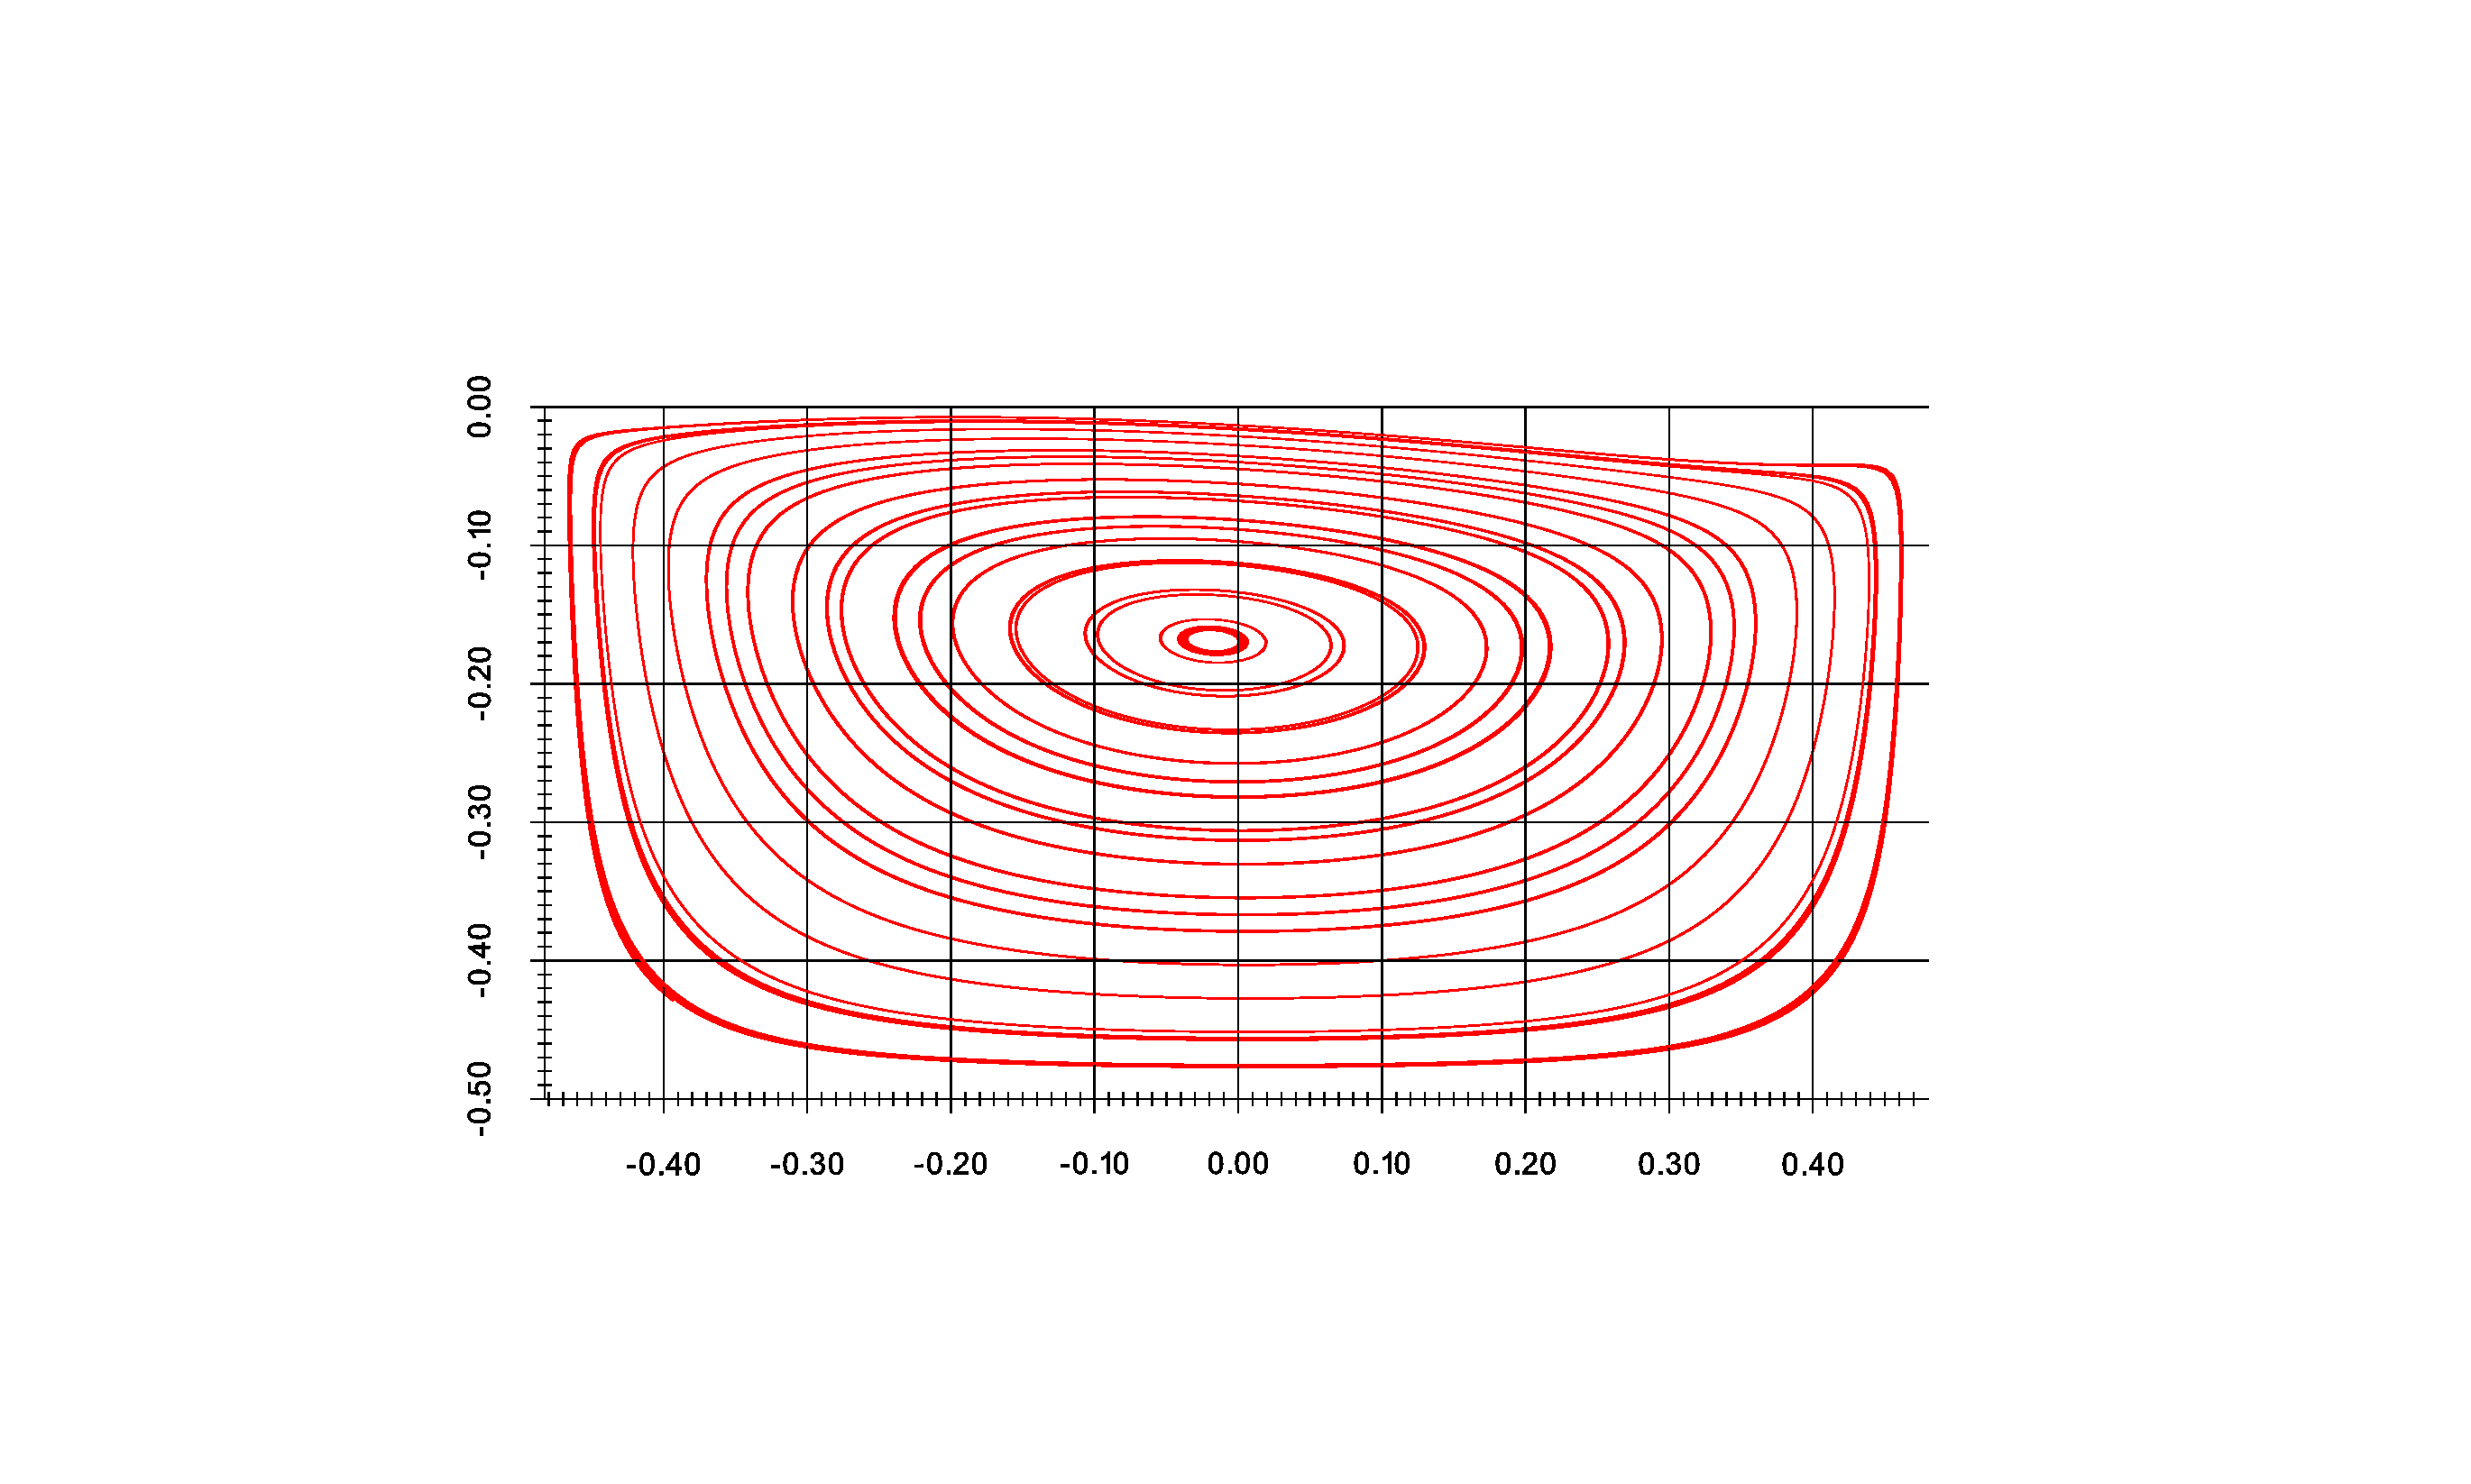
\includegraphics[width=0.5\textwidth]{figure/AR0.5-Re100 streamFunction axis final.pdf}
\caption{AR=0.5, Re=100}
\label{}
\end{center}
\end{figure}

\begin{figure}[tb]
\begin{center}
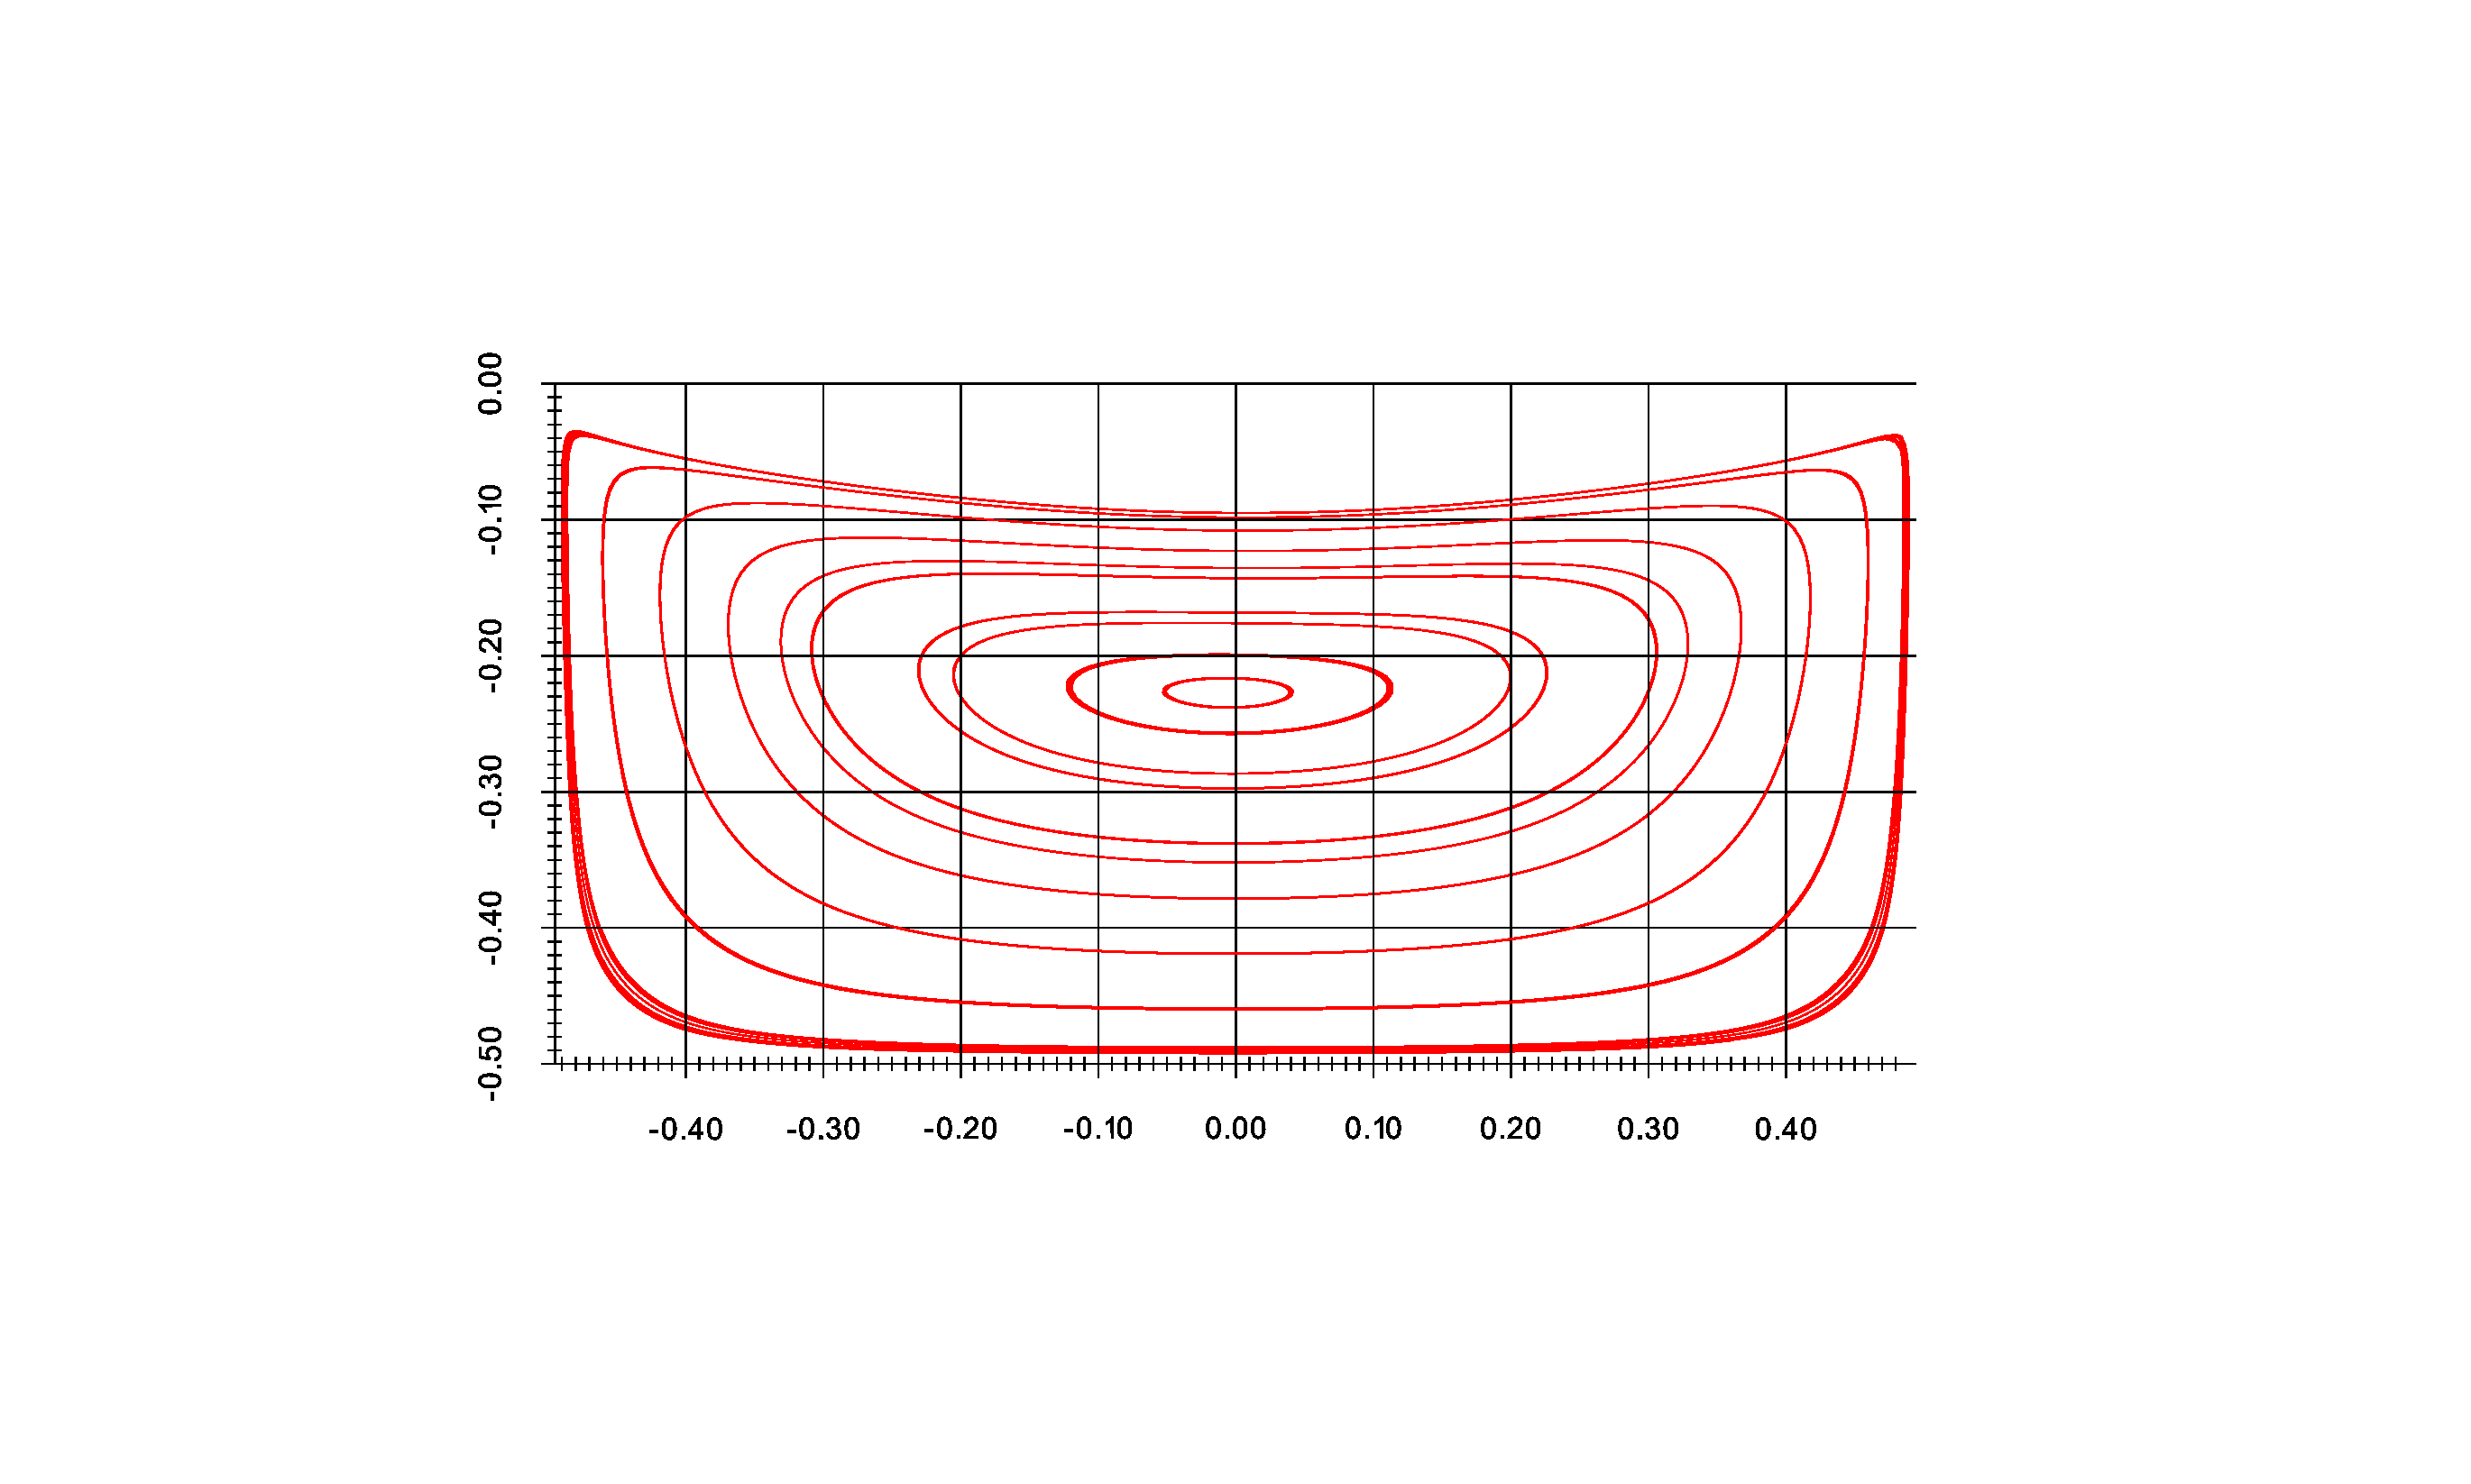
\includegraphics[width=0.5\textwidth]{figure/AR0.5-Re1 streamFunction axis final.pdf}
\caption{AR=0.5, Re=1}
\label{}
\end{center}
\end{figure}

\begin{figure}[tb]
\begin{center}
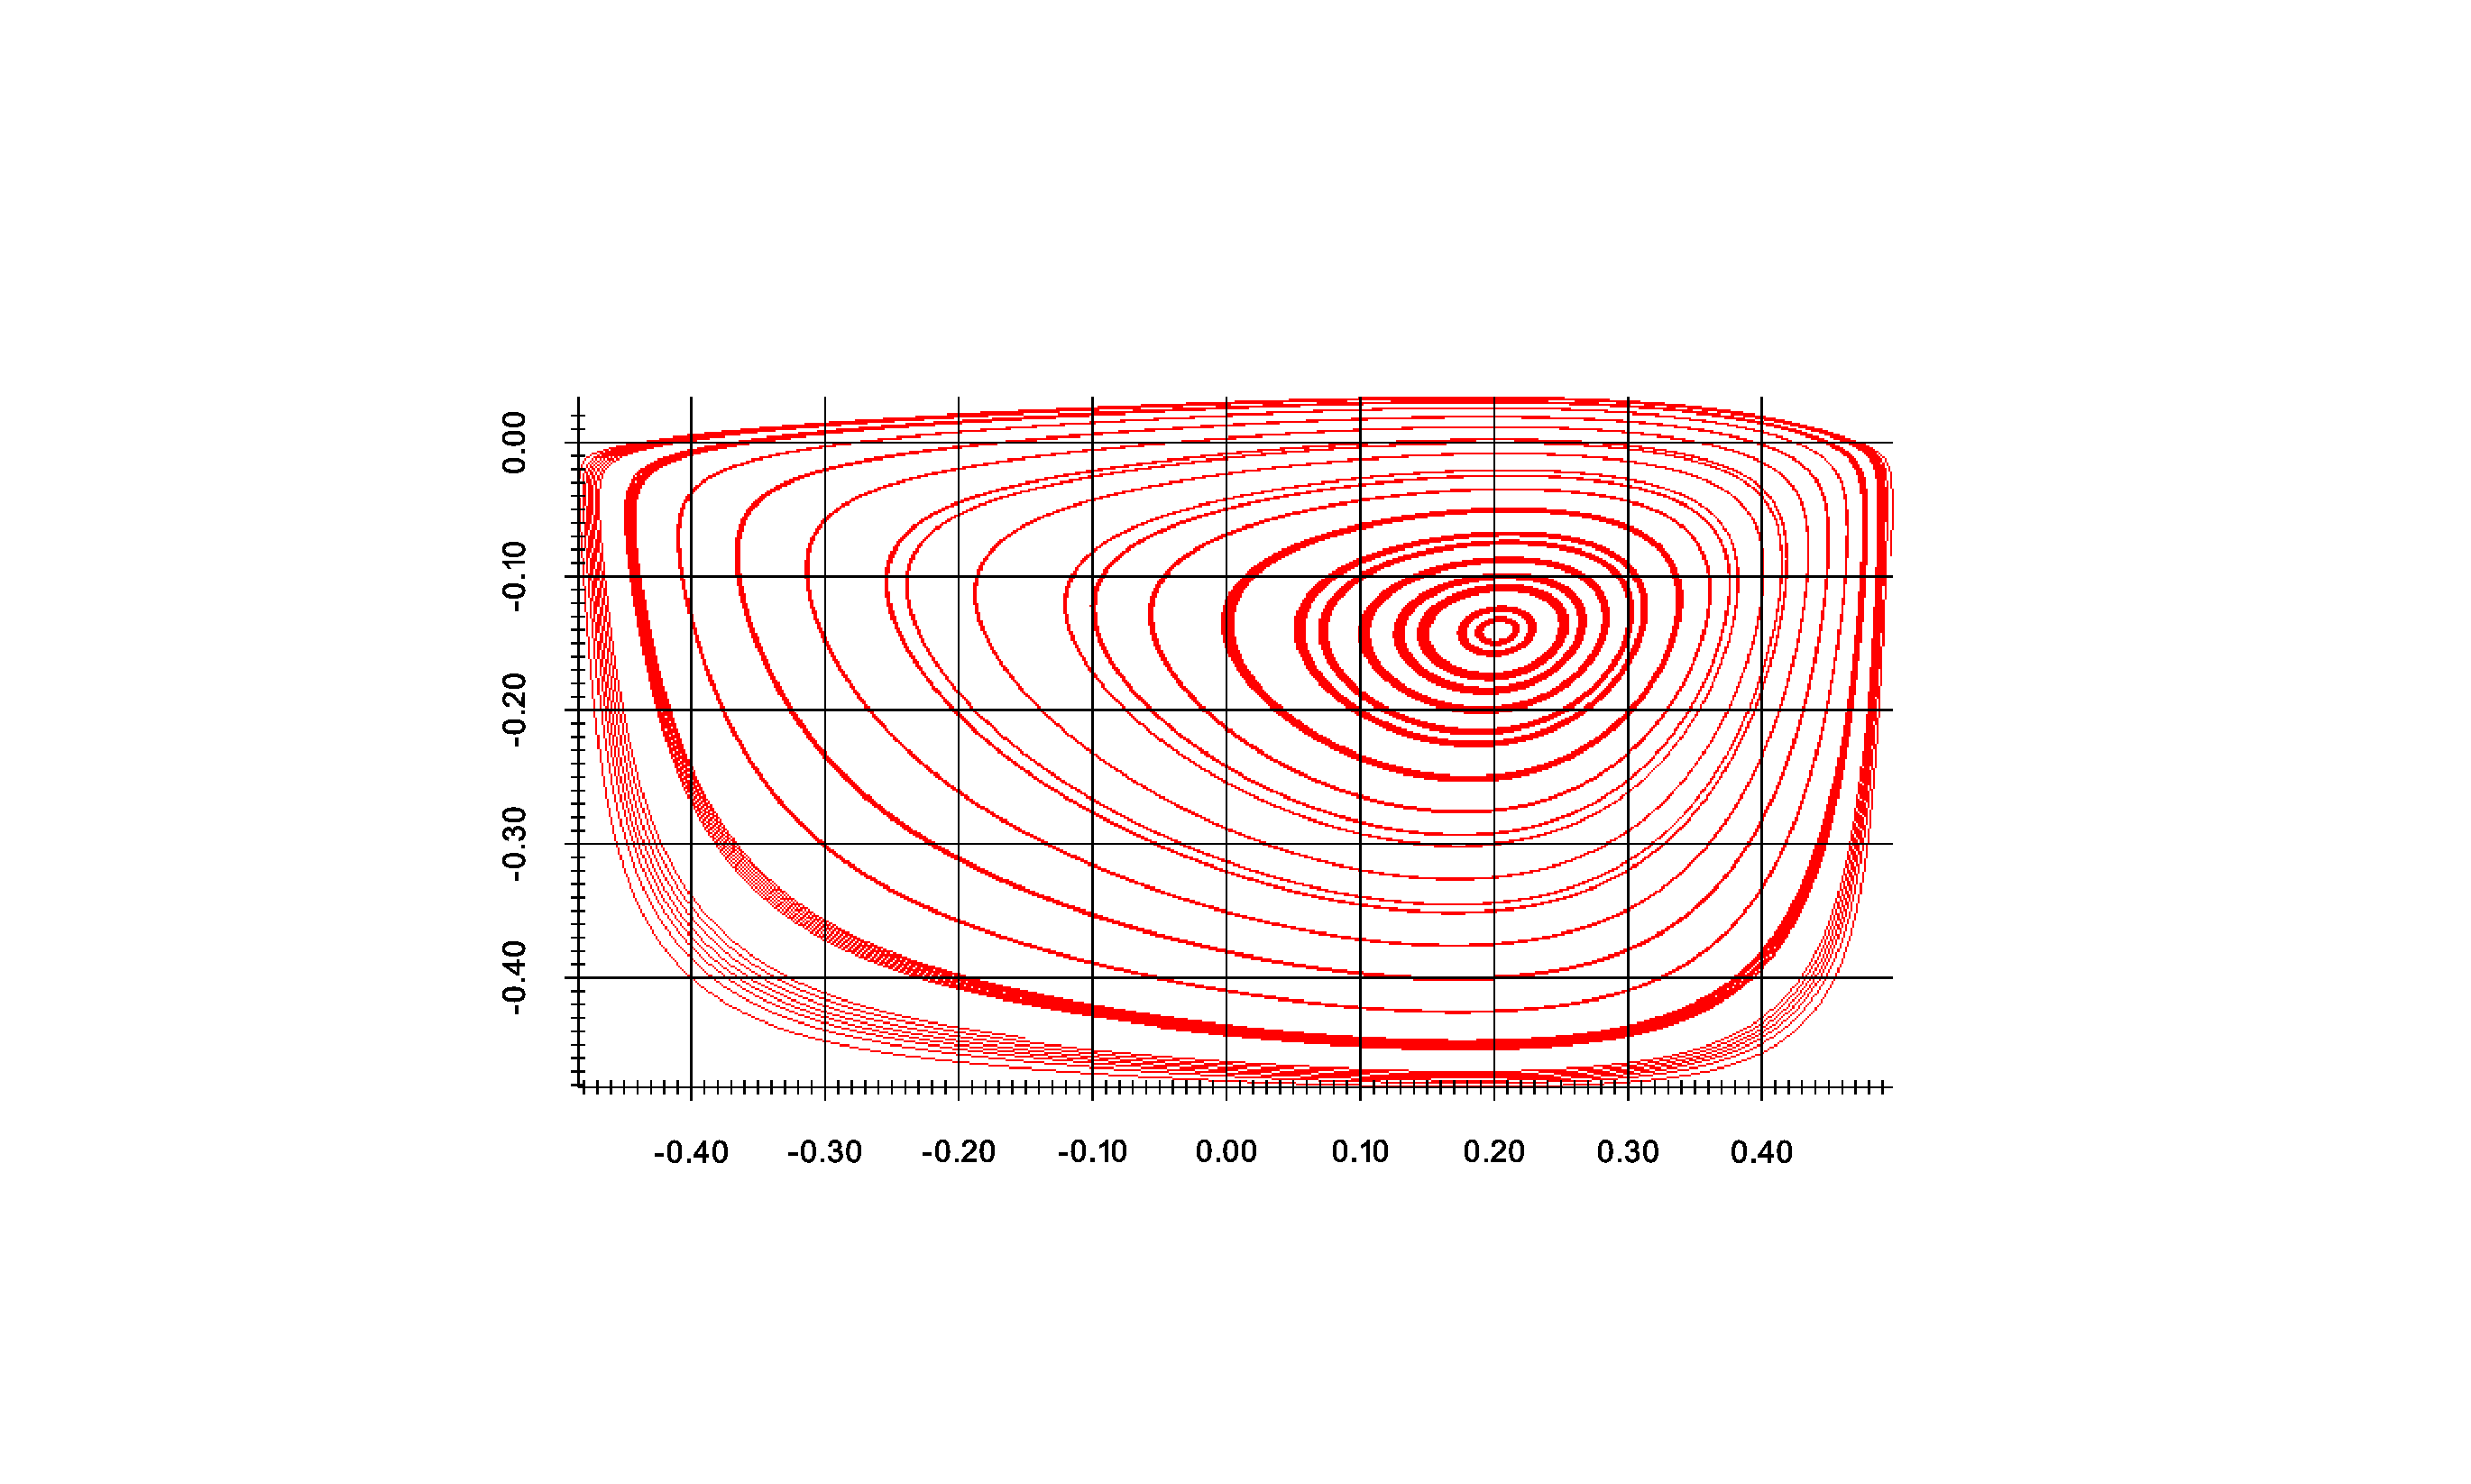
\includegraphics[width=0.5\textwidth]{figure/AR0.5-Re2000 streamFunction axis final.pdf}
\caption{AR=0.5, Re=2000}
\label{}
\end{center}
\end{figure}

\begin{figure}[tb]
\begin{center}
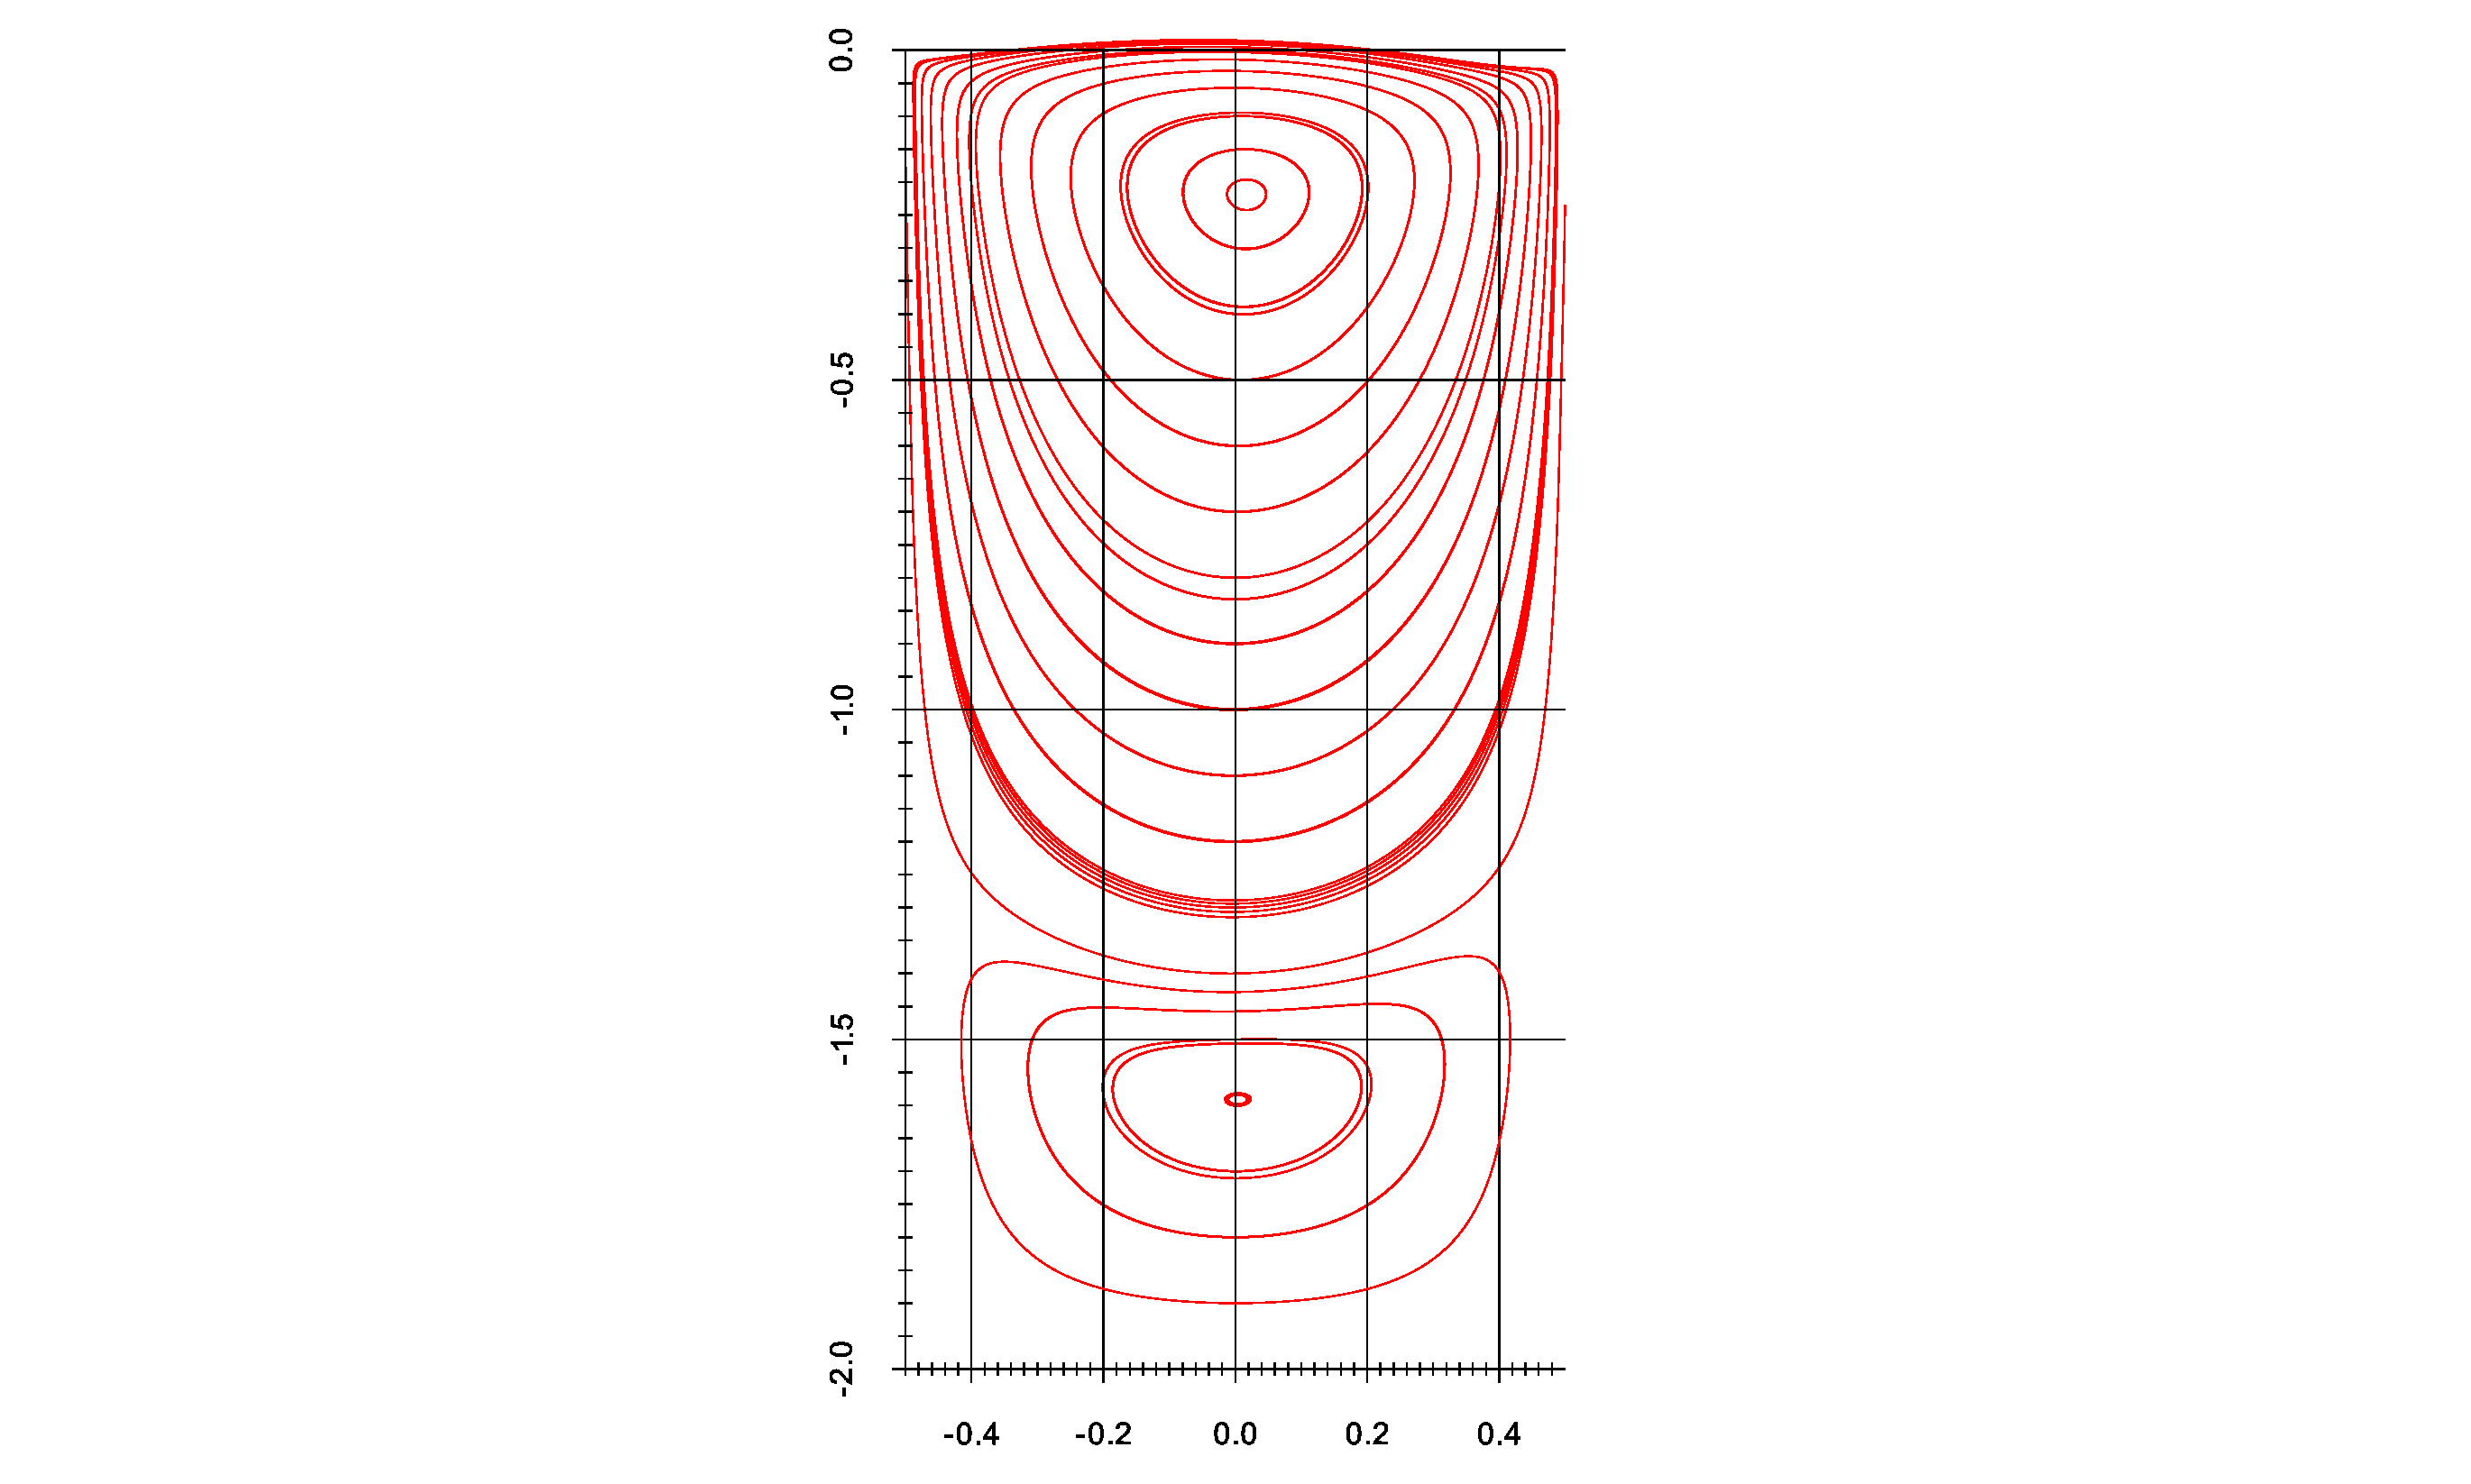
\includegraphics[width=0.5\textwidth]{figure/AR2-Re100 streamFunction axis final.pdf}
\caption{AR=2, Re=100}
\label{}
\end{center}
\end{figure}

\begin{figure}[tb]
\begin{center}
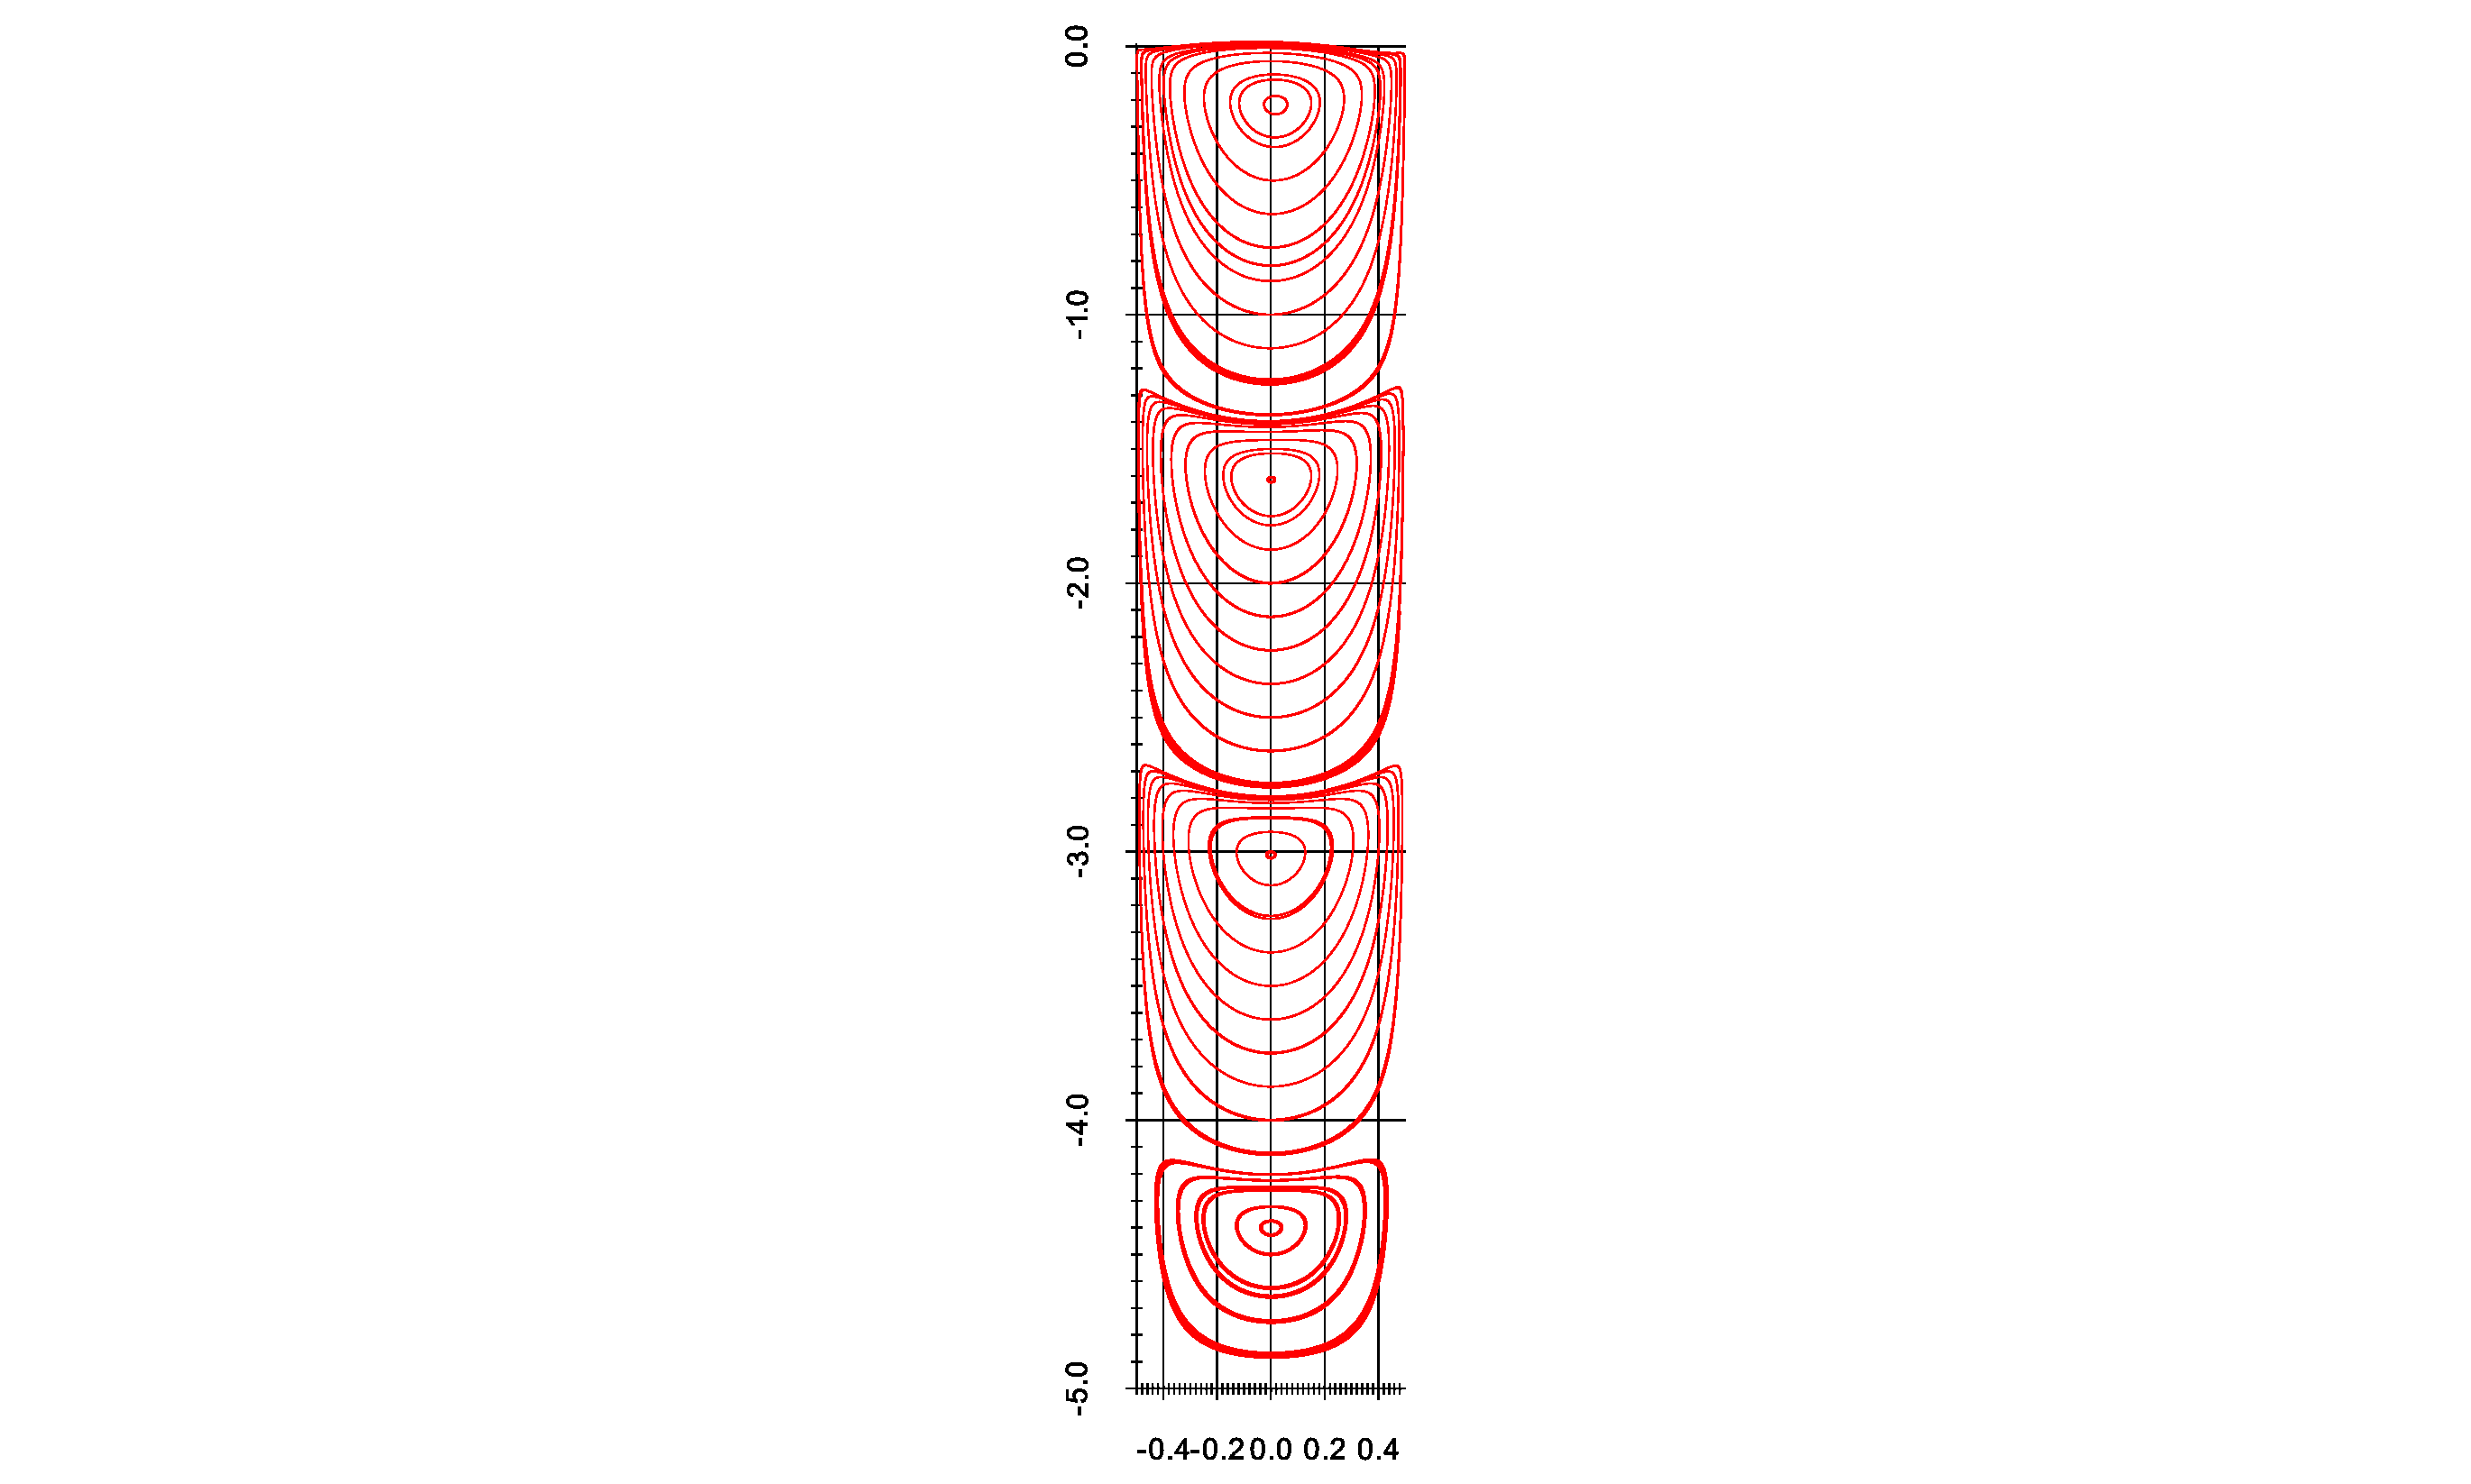
\includegraphics[height=1.4\textwidth]{figure/AR5-Re100 streamFunction axis final.pdf}
\caption{AR=5, Re=100}
\label{}
\end{center}
\end{figure}


%%%%%%%%%%%%%%%%%%%%%%%%%%%%%%%%%%%%%%%%%%%%%%%%%%%%%%%%%%%%%%%%%%%%%%
\section{Results Discussion}

%%%%%%%%%%%%%%%%%%%%%%%%%%%%%%%%%%%%%%%%%%%%%%%%%%%%%%%%%%%%%%%%%%%%%%
\section{Conclusion}

%%%%%%%%%%%%%%%%%%%%%%%%%%%%%%%%%%%%%%%%%%%%%%%%%%%%%%%%%%%%%%%%%%%%%%
\nocite{*}
\bibliographystyle{asmems4}
\bibliography{asme2e}

%%%%%%%%%%%%%%%%%%%%%%%%%%%%%%%%%%%%%%%%%%%%%%%%%%%%%%%%%%%%%%%%%%%%%%
\clearpage
\onecolumn
\appendix       %%% starting appendix
\section*{Appendix A: Python Code}

\lstinputlisting[caption=Code to create solutions, language=Python]{../code/Final.py}

%%%%%%%%%%%%%%%%%%%%%%%%%%%%%%%%%%%%%%%%%%%%%%%%%%%%%%%%%%%%%%%%%%%%%%
\end{document}
